\chapter{Related Work}
\label{sec:rw}

This chapter discusses design (focusing on rapid fabrication and laser
cutting) and research on physical and computationally-supported
sketching.

\section{Design for Rapid Fabrication}

A growing community of self-described \textit{makers} design and build
many kinds of physical things~\cite{gershenfeld-fab}. Some are
electronic or robotic gizmos, while others are made from traditional
craft material. These ``new makers''~\cite{gross-new-makers} are
empowered by rapid fabrication machines like 3D printers and laser
cutters.

It is possible that we are beginning to see a shift from an economy
based on mass-production (in factories) to one that includes
mass-customization (in homes, schools, and community
centers)~\cite{economist-fab}. Rapid fabrication machines continue to
decline in price while improving in quality. A new sector of
businesses use rapid fabrication to cater to the needs of hobbyist
designers as well as people that need highly customized
goods~\cite{paulos-citizenscience}. For example, companies such as
Ponoko fabricate and send users physical output based on digital
models uploaded over the web.

Rapid prototyping machines are used in many domains: mechanical
engineering, architecture, craft work, industrial design---just to
name a few. While many users of these machines are professional, a
growing population of Makers are not necessarily educated (in a
traditional sense) to design and build things. Instead, members of
this group might be better described as hobbyists or
semi-professionals. They are smart and motivated, but do not
necessarily have a great abundance of time or money.

\subsection{Rapid Fabrication Machines}

The software modeling tool discussed later in this thesis targets
laser cutters, which are one particular type of rapid fabrication
machine. I will first describe the broader area of rapid fabrication
to situate the specific machine in question.

There are several related (but not necessarily interchangeable) names
for machinery to in this space. \textit{Numerical Control (NC)}
machines were introduced in the 1950s that ran programs encoded on
punched tape. \textit{Computer Numerical Control (CNC)} introduces a
computer, capable of performing conditional execution soon
followed. Modern CNC machines are found anywhere from large automobile
factories (e.g. as sophisticated robots) to the home-brewed 3D printer
set up in the hobbyist's garage.

When applied to CNC machines, the terms ``rapid fabrication'' and
``rapid prototyping'' refer to their role in a design process. While
industrial CNC robots are engaged in large-scale production work,
rapid fabrication machines are used primarily by designers to explore
ideas and construction (preceding large-scale production, if it
happens at all). Because of their role in the design process it is
critical that these devices are faster and cheaper than using human
labor with manual machinery.

The type, quality, and composition of the output depends not only on
the machine, but also on the designer's skill in creating suitable
instructions. A CNC mill, for example, could be used to create a
customized office desk. But in order to build the parts comprising the
desk, somebody must give the machine a digital model that indicates
not only where the mill will cut, but how the cut will be made.

A mill may operate with 3 or more axes: it can move on the x/y plane,
and up and down (z-axis). Some models have additional axes that allow
the tool head to move in other ways, such as rotation. The tool path
is therefore an important consideration when designing for most types
of computer controlled manufacturing machines. In many (but not all)
cases, software tools can compute tool paths automatically. Designers
must consider a machine's capabilities.

Laser cutters can be thought of as a very fast, strong, and precise
automated razor blade, cutting through flat material (paper, wood,
plastic, metal, etc.) from directly above. Many items can be made
entirely with a laser cutter, aside from the occasional screw or glue.

SIMI targets design for laser cutters. This tool was chosen for
several reasons. First, problems related to tool paths are nearly
non-existent. Second, a laser cutter executes quickly, which supports
a faster loop of coding, testing, and debugging. Fabricating a
toothbrush holder takes about five minutes on a typical laser cutter,
but a 3D printer would take four hours to make a similar object. Last,
laser cutters are among the more popular rapid fabrication machines.

Laser cutter users place material on the laser cutter's \textit{cut
  bed}. Typical sizes for cut beds are in the range of 12''x 18'' to
48'' x 72'' (30 x 46 cm to 122 x 183 cm). A laser is directed through
several mirrors mounted on robotic arms. These arms move to allow the
laser to reach any location on the cut bed. A lens near the end of the
path focuses the laser to the material to create an optimal cut. A 40
watt machine can cut $\frac{1}{4}''$ (6mm) thick wood; a 100 watt
machine can cut up to 1'' (25mm) plywood.

\subsection{Current Design Tools for Laser Cutting}

Today, designers can choose among several modeling tools for laser
cutter projects. The most commonly used tool is Adobe Illustrator, a
general-purpose vector graphics editor. It is full-featured and has an
interface new users find familiar, as it presents interaction with
menus, tool bars, and persistent tool modes. However, participants in
our formative study (presented later in
Section~\ref{sec:formative-interviews}) had a hard time using
Illustrator quickly and effectively because they spent a great deal of
effort looking for appropriate functions among the many features that
are irrelevant to laser cutters. 

Specialized CAD tools like Rhino or SolidWorks (see
Figure~\ref{fig:cad-screenshots}) are perhaps more appropriate for
this kind of modeling but they also have a substantial learning
curve. If rapid fabrication is to become common, appropriate modeling
tools must be made accessible to ordinary
users~\cite{lipson-homefactory}.

\begin{figure}
  \centering
  \begin{subfigure}[t]{0.42\textwidth}
    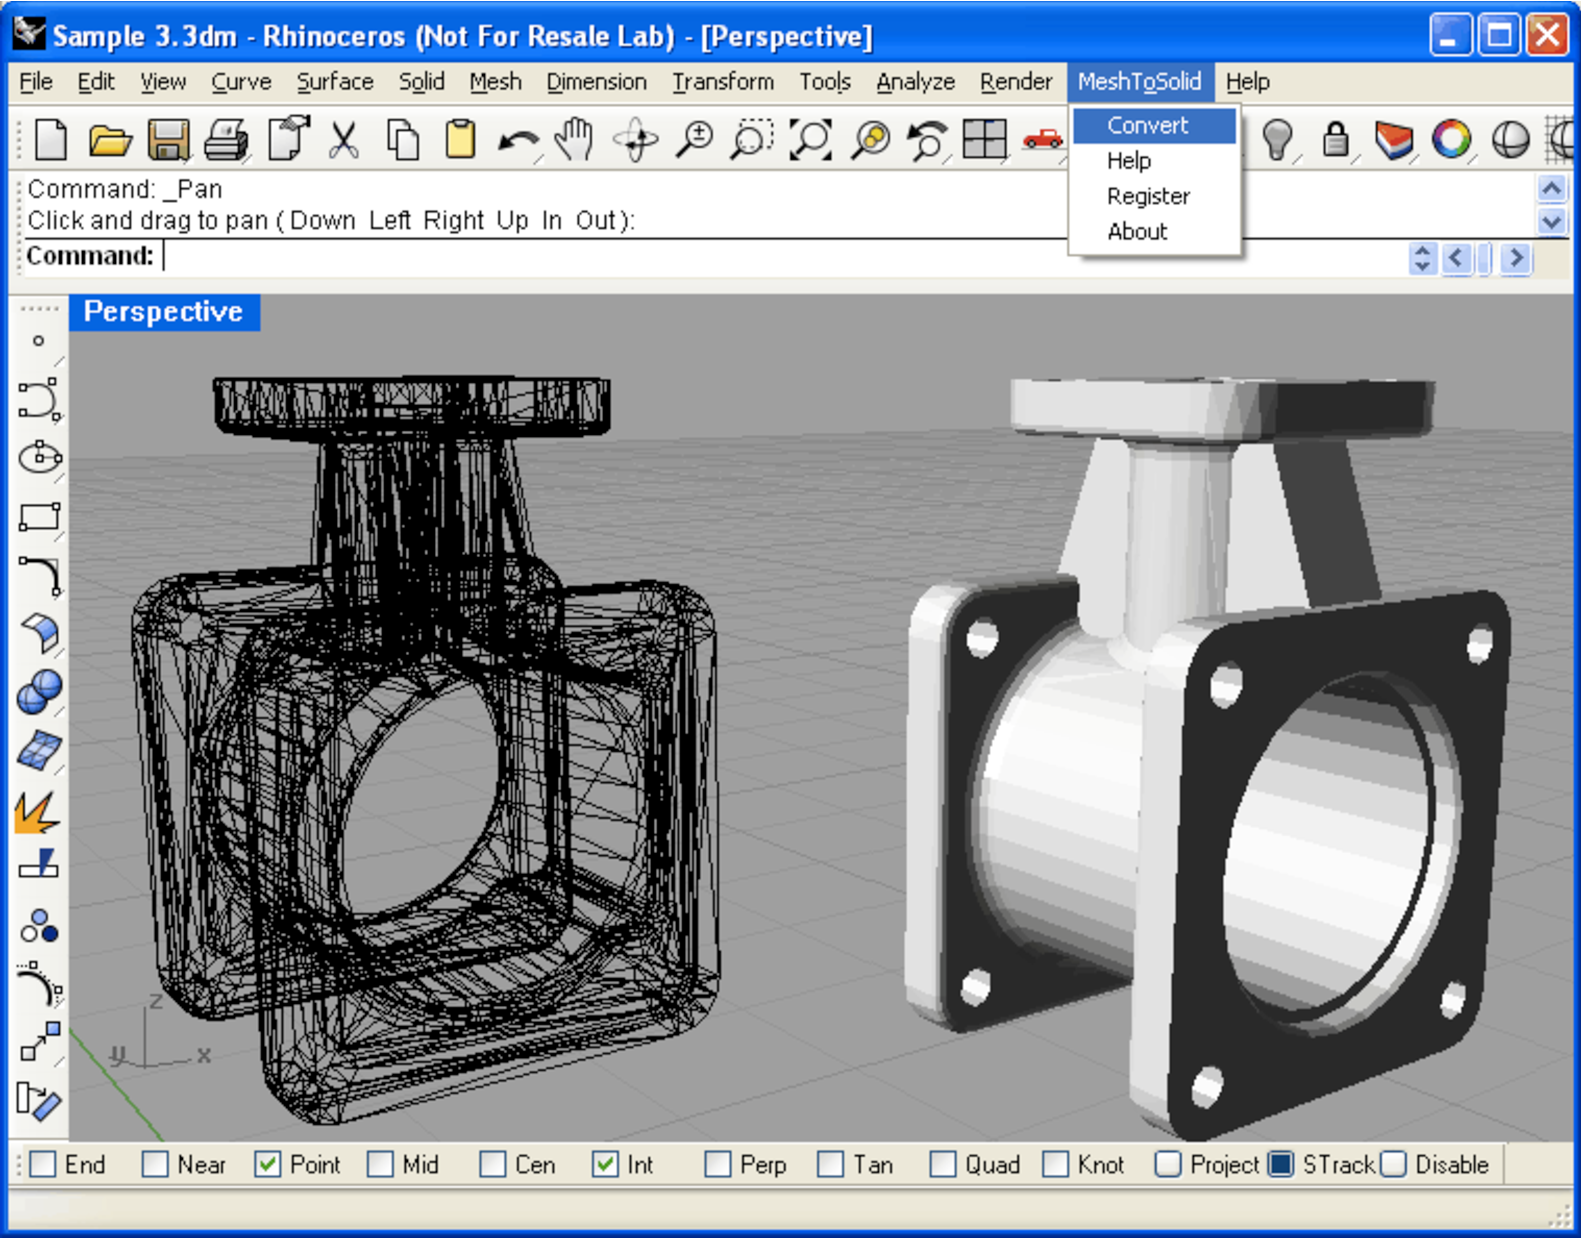
\includegraphics[width=\linewidth]{img/rhino3d-screenshot.pdf}
    \caption{Rhino 3D modeling software.}
    \label{fig:rhino3d-screenshot}
  \end{subfigure}
  \hspace{1cm} % spacing, do what you need
  \begin{subfigure}[t]{0.42\textwidth}
    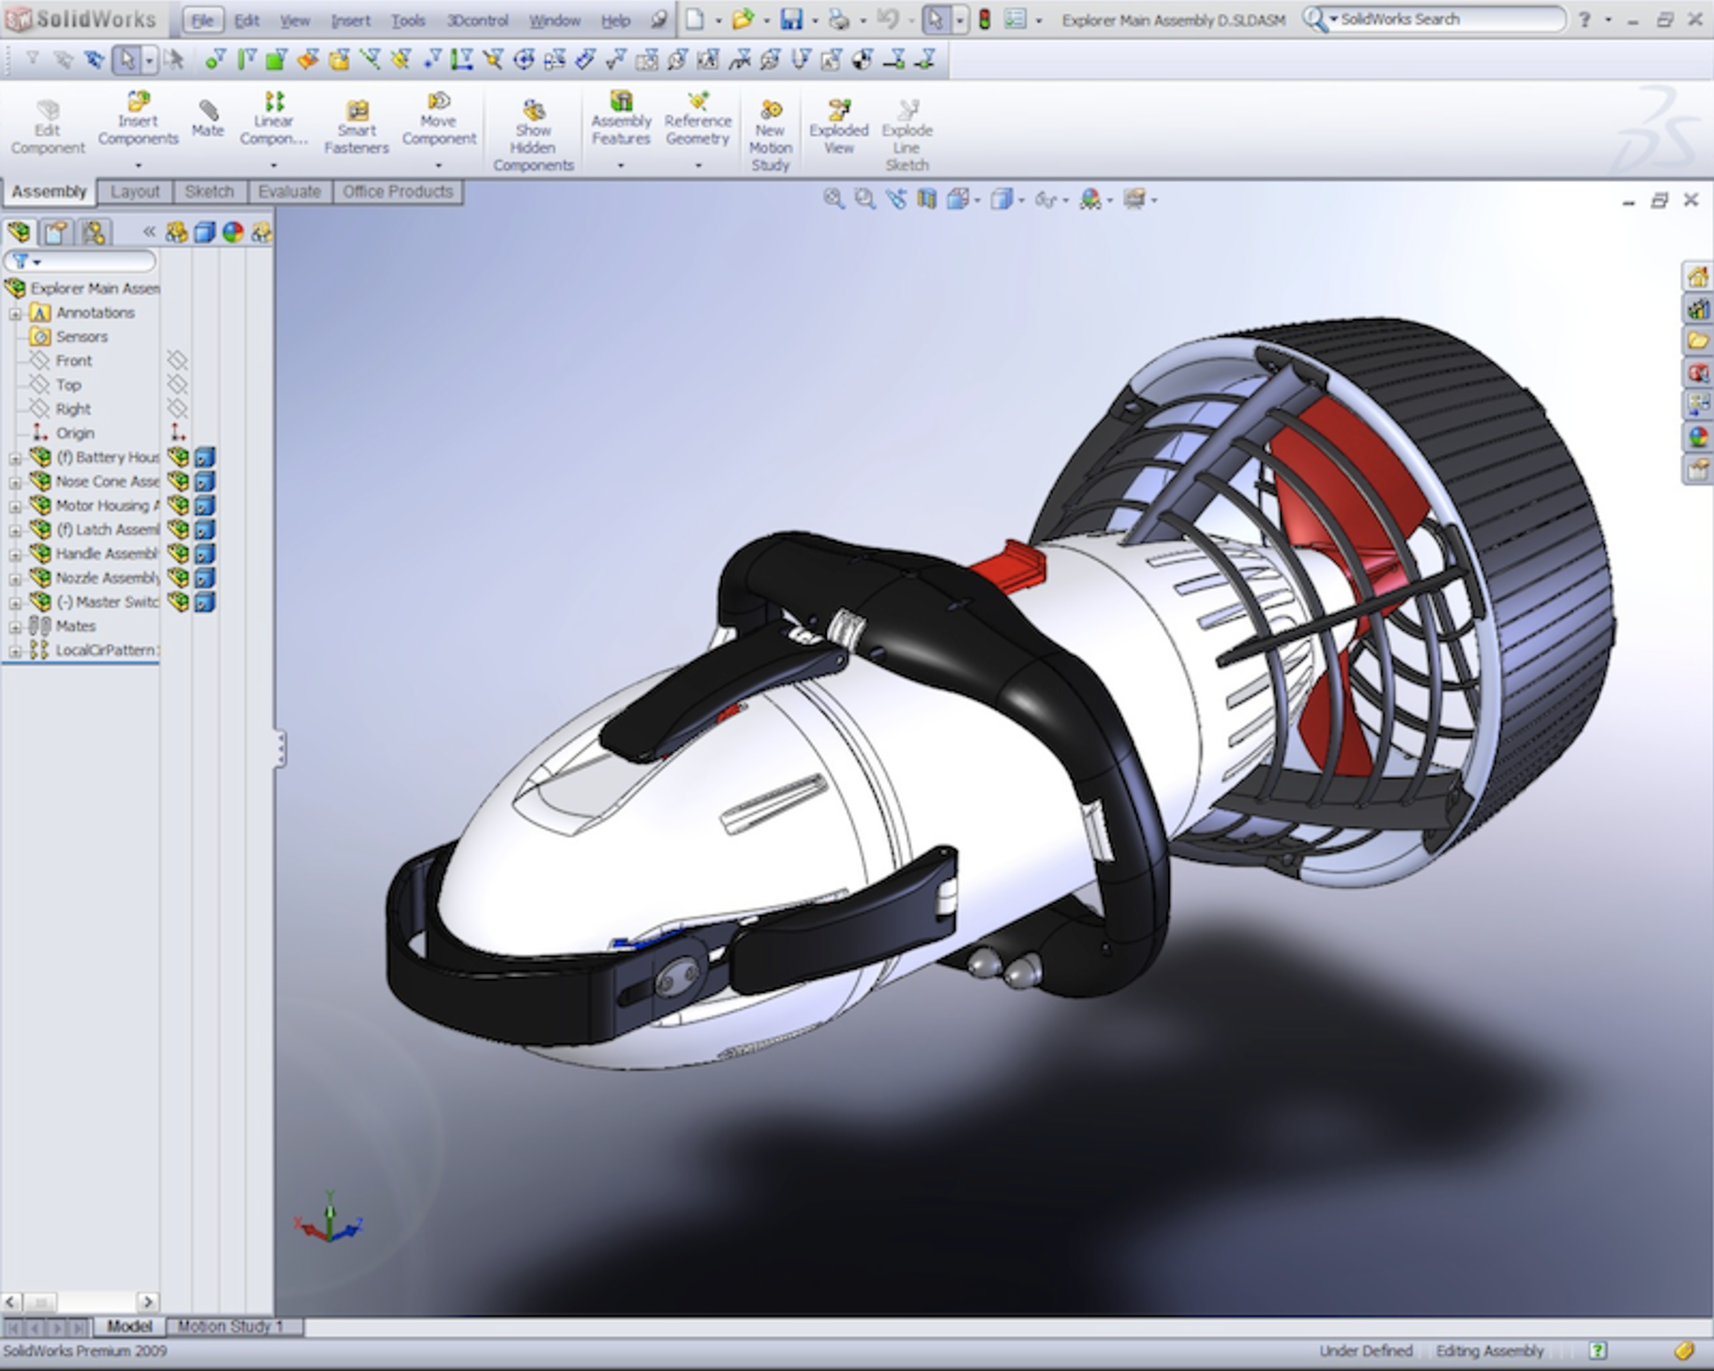
\includegraphics[width=\linewidth]{img/solidworks-screenshot.pdf}
    \caption{Solidworks modeling tool.}
    \label{fig:solidworks-screenshot}
  \end{subfigure}
  \caption[Advanced 3D CAD Software]{Rhino 3D and Solidworks are two commonly used 3D modeling tools and are often used by skilled users for various rapid fabrication purposes, including laser cutting.}
  \label{fig:cad-screenshots}
\end{figure}


\section{Design Sketching}

People commonly sketch when problem solving. Some sketches are
personal, others collaborative. Some help people make quick
calculations and are quickly forgotten while others serve longer-term
purposes. For professional designers, sketching is a \textit{process}
to think about problems. Just as importantly, a sketch (the result of
the process) is a \textit{record} that communicates
ideas~\cite{ferguson-engineering}.

Design can be seen as an iterative process of problem-framing and
exploring possible solutions within the current conception of the
problem. A sketch is not a contract: it is a proposal that can be
modified, erased, built upon. The rough look of hand-made sketches
suggests their provisional nature.

Some theories of cognition give the human mind two distinct tasks: to
perceive the world via our senses, and to reason about what our senses
provide. In contrast, the late psychologist Rudolf Arnheim argues that
perception and thinking are inseparable: ``Unless the stuff of the
senses remains present the mind has nothing to think
with''~\cite{arnheim-visthink}. Visual thinking is valuable in
evaluating what is and designing what might be. Sketching allows
people to give form to notions that are otherwise imaginary; the act
of seeing fuels the process of reasoning.

Sketching plays a crucial role in the practice of design. It helps
people think about problems and offers an inexpensive but effective
way to communicate ideas to others. The practice of sketching is
nearly ubiquitous: One recent study of interaction designers and HCI
practitioners found that 97\% of those surveyed began projects by
sketching~\cite{myers-behavior-design}. We must understand the purpose
and practice of sketching as it is done \textit{without} computation
if we hope to effectively support it \textit{with} computation.

% Karolina's project management and Shaun's floor plan diagram.
\begin{figure}
  \centering
  \begin{subfigure}[b]{0.42\textwidth}
    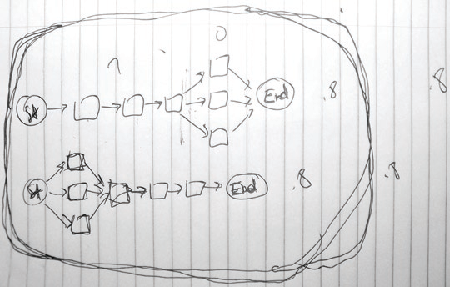
\includegraphics[width=\linewidth]{img/sketch-type-project-management.pdf}
    \caption{Project management diagram showing task precedence of two
      projects. Hastily drawn boxes and arrows represent abstract
      activities.}
    \label{fig:sketch-type-pm}
  \end{subfigure}
  \hspace{1cm}
  \begin{subfigure}[b]{0.42\textwidth}
    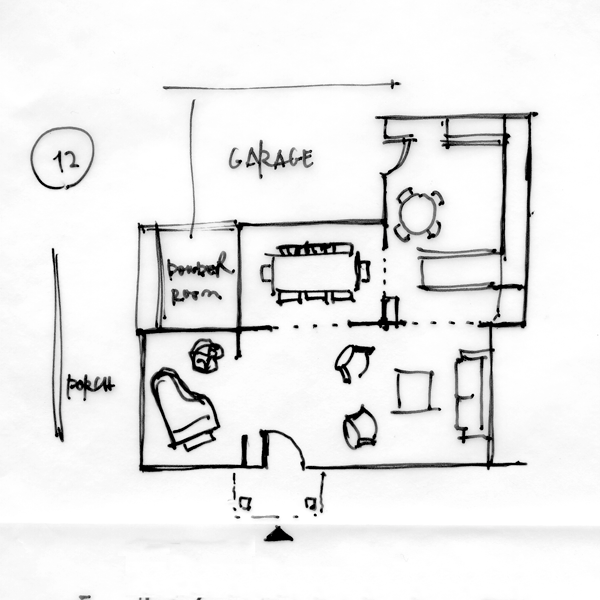
\includegraphics[width=\linewidth]{img/sketch-type-architecture.pdf}
    \caption{An architect's floor plan sketch. It includes text, 
      spatial information, and symbols representing household
      items like a piano or dining table.}
    \label{fig:sketch-type-architecture}
  \end{subfigure}
  
  \caption[Project Management and Architecture Sketches]{Sketches vary
    in domain and in the visual characteristics of marks.}
  \label{fig:types-of-sketches}

\end{figure}


While designing, we iteratively explore and refine the problem
definition and proposed solutions. Sketching supports this creative
search process. We set out on our design task with some high-level
goals. However, due to the
ill-structured~\cite{simon-ill-structured-problems} and ``wicked''
nature of design~\cite{rittel-wicked}, we encounter unforeseen
opportunities and constraints as designing progresses. Those
opportunities and constraints may be implicit in the original problem
description, but designers expose them as they explore. The
discoveries are incorporated into the understanding of the problem and
potential solutions. Design problems are ``not the sort of problems or
puzzles that provide all the necessary and sufficient information for
their solution~\cite{cross-nature-nurture}.'' So it goes with
sketching. We draw different views of our model, which allows us to
perceive the problem in new ways.

Designers engage in a sort of ``conversation'' with their sketches in
a tight cycle of drawing, understanding, and
interpreting~\cite{schon-kinds-of-seeing}. Goldschmidt describes this
as switching between two reasoning modes: ``seeing that'' and ``seeing
as''~\cite{goldschmidt-dialectics}. \textit{Seeing that} is the
process of recognizing the literal, descriptive properties of the
drawing. \textit{Seeing as} is figurative and transformative, allowing
the designer to re-interpret parts of the sketch in different
ways. Care must be taken to support this conversation when developing
sketch-based modeling tools. If the system interprets drawings too
aggressively or at the wrong time, it may prevent the human designer
from seeing alternative meanings; recognize too little and the
software is no better than paper.

\subsection{Prototyping and Fidelity}
\label{sec:traditional-prototyping}

Newman and Landay's ethnographies of web designers focused on how
designers use informal techniques~\cite{newman-web-designers}. They
found that designers always sketch at the beginning of a web design
project, exploring numerous high-level options. Frequently this early
sketching phase is accompanied with construction of low-fidelity
prototypes made on paper or with simple software tools like Microsoft
PowerPoint. As the design progresses and designers incrementally add
details, they move to higher fidelity models. Client meetings are an
important forcing function in web design projects. When meeting with
clients, designers want to show polished prototypes produced with
computer software. Therefore designers used electronic tools earlier
in the process than they would otherwise have preferred.

Today most software tools support incremental refinement and
specification of details but do not adequately support idea generation
or exploration~\cite{terry-creative-ui}. Designers who begin using
software tools in the early phases of design tend to make superficial
explorations of possible solutions. Further, because tools are poor
for exploration but good for specifying details (font, line weight,
and color), designers tend to focus on nuances that are not yet
important. Observing that current tools are inadequate for creative
pursuits, researchers have developed calligraphic tools such as SILK
and DENIM, which aim to support the early phases of
design~\cite{landay-silk,lin-denim}.

Paper sketches dominate the early phases of design as people generate
new ideas, in a process Goel terms ``lateral
transformations''~\cite{goel-sketches-of-thought}. But as soon as the
web designer believes he or she will make incremental revisions (which
Goel calls ``vertical transformations'') they switch to a computer
tool.

\subsection{Sketches as a Symbol System}

% Cartoon clouds or trees: Overloaded, Ambiguous
\begin{figure}
  \centering
  \begin{subfigure}[b]{0.3\textwidth}
    \centering
    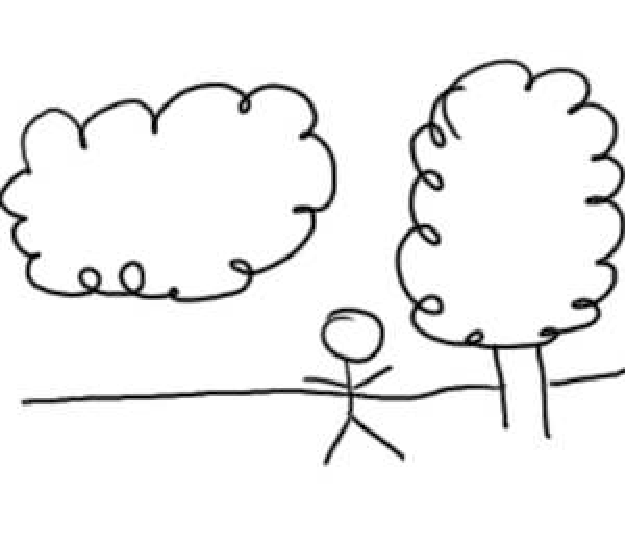
\includegraphics[width=\textwidth]{img/cloud-1.pdf}  
    \caption{Overloaded semantics: The cloud and tree have similar
             shapes but different meanings due to context.}
    \label{fig:cloud-1} 
  \end{subfigure}
  \hspace{0.03\linewidth}
  \begin{subfigure}[b]{0.3\textwidth}
    \centering
    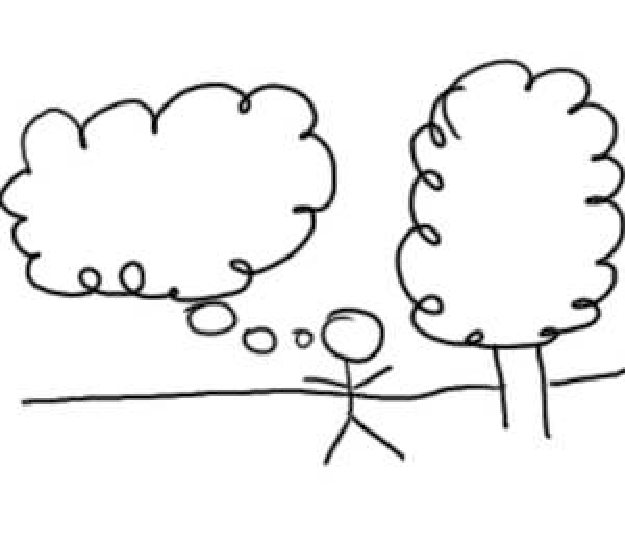
\includegraphics[width=\textwidth]{img/cloud-2.pdf}  
    \caption{Ambiguity: A small addition changes our
      interpretation. The object at left may be a cloud or a thought
      bubble.}
    \label{fig:cloud-2} 
  \end{subfigure}
  \hspace{0.03\linewidth}
  \begin{subfigure}[b]{0.3\textwidth}
    \centering
    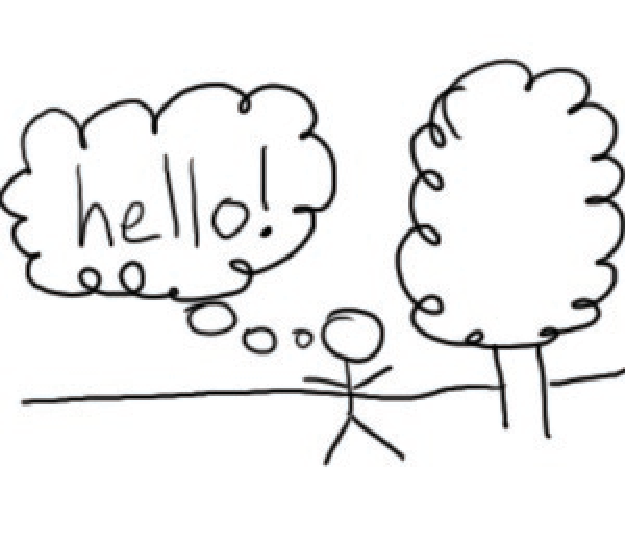
\includegraphics[width=\textwidth]{img/cloud-3.pdf}  
    \caption{More information gives more confidence about object
      identity. Text in the cloud indicates a thought bubble.}
    \label{fig:cloud-3} 
  \end{subfigure}

  \caption[Overloaded semantics and ambiguity]{Overloaded semantics
    and ambiguity.}
  \label{fig:cloud}
\end{figure}


Goodman provides a comprehensive framework for analyzing the
properties of various symbol systems, including
sketches~\cite{goodman-symbols}. Goel places sketching in Goodman's
framework, noting that sketches have \textit{overloaded semantics},
they are \textit{ambiguous}, \textit{dense}, and
\textit{replete}~\cite{goel-sketches-of-thought}. These properties
describe one particular sense of sketching in which the drawer's marks
may be idiosyncratic. It is critical to understand these properties
when developing sketch-based design software.

Sketches have ``overloaded semantics'': The same symbol may mean
different things depending on context. Further, a sketched symbol may
be ``ambiguous'', meaning that the symbol affords more than one
plausible interpretation.  Figure~\ref{fig:cloud} illustrates these
properties. A lumpy shape can be used to indicate many things
including clouds, trees, or thought bubbles. We interpret the shape
differently depending on context.

Sketched symbols are ``dense'', indicating there is a continuous range
between instances of the same symbol. While there may be minute visual
discrepancies between symbol instances, Goel claims that such symbols
are also ``replete'': no aspect of the sketched symbol may be safely
ignored (Figure~\ref{fig:dense-replete}).

The pen strokes constituting a sketch serve various functions. Ink may
indicate abstract domain symbols (e.g. diode, treble clef), object
boundaries, actions (e.g. arrows indicating containment or movement),
dimensions and units, annotations, region texturing, and so on. Some
parts of a sketch are more dense and replete than others. For example
a diode's properties do not change if it is drawn with a slightly
larger triangle. However, subtle variations in how a desk lamp is
drawn might lead to substantially different esthetic responses to it.

% Stick figures: dense and replete
\begin{figure}
\begin{center}
  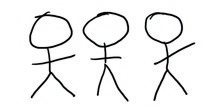
\includegraphics[angle=0, origin=c, width=6cm]{img/dense-replete-stick-figures.pdf}
  \caption[Dense and replete sketches]{Different instances of the same
    stick figure vary along a continuum (\textit{dense}). However, the
    visual properties of individual symbols may (or may not)
    communicate additional information (\textit{replete}). Is the
    figure at the right waving? }

  \label{fig:dense-replete}
\end{center}
\end{figure}


Gross and Do discuss some properties of hand-drawn diagrams from the
perspective of building tools to support design drawing
activities~\cite{gross-ecn-uist}. The authors distinguish sketches
from diagrams, noting that diagrams are ``composed of primitive
elements chosen from a small universe of simple symbols---boxes,
circles, blobs, lines, arrows.'' This list is certainly not
exhaustive, but it does illustrate the general idea that diagrams have
a limited vocabulary. In practice, sketches and diagrams from various
dialects may be combined (e.g. mathematical notation on the same page
as circuit diagrams and hand written notes.)

Freehand diagrammatic drawings are abstract, ambiguous, and
imprecise. \textit{Abstract} symbols denote elements whose identities
or properties are not (yet) important or known. For example,
Figure~\ref{fig:sketch-type-pm} on page \pageref{fig:sketch-type-pm}
shows a project management diagram of two hypothetical projects. The
activities composing each project are abstract---they could represent
anything. The value of the project sketch is that it shows the network
structure and does not draw attention to what specific activities are.

An \textit{ambiguous} symbol has many plausible interpretations. The
floor plan sketch in Figure~\ref{fig:sketch-type-architecture} shows
several rectangles indicating rooms, furniture, shelves, or
counters. Human observers can confidently disambiguate the intended
meaning of some rectangles, but others remain unclear. The
bottom-right of the sketch shows two armchairs and a sofa with an
ambiguous rectangle in the middle that could plausibly represent
either a rug or a coffee table.

Last, freehand diagrams are \textit{imprecise}. Imprecision allows
designers to work with rough values (e.g. ``about two meters wide'')
and avoid premature commitment. Imprecision also indicates that the
design is by no means final.

The notational properties of sketches make them powerful tools for
supporting visual thinking. Designers may leverage ambiguities in
their sketches to see new meanings, for example. However, these same
properties present challenges for accurate software recognition.

The degree to which a drawing is ambiguous, imprecise, and abstract
varies among instances, and people might interpret them differently. A
rough sketch is useful to designers, especially for brainstorming and
incremental development of ideas. But in order for the sketch to be
transformed into a finished product (e.g. as a digital model supplied
to a rapid manufacturing device), it must be made unequivocal,
precise, and concrete. The process of moving from the informal sketch
to the formal specification involves drawings that are semi-ambiguous,
partially precise, and with some abstractions given definite
identities.

\subsection{Summary: Traditional Sketching and Computation}
\label{ref:traditional-summary}

If we hope to effectively support sketching with computation, we must
first understand the practical aspects of traditional sketching. 

Sketching is an important---perhaps necessary---tool for doing
design. It gives a way to quickly make provisional drawings, which
help us efficiently make sense of spatial, relational
information. Sketches let us make marks that are as vague or specific
as needed. Because sketched elements can be ambiguous, rough drawings
have different interpretations. We may reflect on sketches to see new
meaning in existing marks. People sketch in part because they don't
know exactly what they are making: sketching facilitates exploration.

Low-fidelity prototypes are especially important as tools to test
ideas during early design. This is because they are easy to make,
allowing designers to quickly expose problems before committing to
decisions. Sketching is a common method of creating such prototypes.

In order for computers to recognize sketches, we must develop
techniques to transform imprecisely made marks into discrete
symbols. However, some of the properties that make a sketch useful for
a human (overloaded semantics, ambiguous, imprecise, etc.) complicate
the task of computer recognition.

%% Be sure to also talking about pragmatic vs. epistemic actions, and
%% the tentative, exploration al nature of design sketching.

\section{Hardware: Tablets and Pens}

Now that I've discussed the role of sketching in design, and some of
the cognitive aspects of freehand drawing, I will now present topics
involved in supporting sketching with computers. This section
discusses hardware people might use to give input to a sketching
system, and the next enumerates software topics for processing it.

Researchers in sketch recognition and interaction typically use tablet
devices such as a Wacom Bamboo or Cintiq. Some surfaces, like the
Bamboo, simply sense stylus input but do not display feedback. These
``blind'' tablets require the user to look at one place (their
computer display) but draw on another surface. This can lead to
hand-eye coordination trouble. The Cintiq, and various Tablet PC
computers, combine display and sensing surfaces. In this case, the
user's pen comes into contact with a drawing plane that is separated
from the display plane by only a few millimeters. When the user views
the display at an angle, this parallax difference can be annoying, but
it is certainly better than the situation with blind tablets.

Input surfaces that are intended to be used with fingers or hands
offer different interaction experiences than pen-oriented drawing
surfaces. For example, users may trace shapes with a single finger,
use two fingers to zoom in or out, or use whole-hand gestures for
issuing other commands. These interaction techniques provide
opportunities for developing innovative sketching applications, as
demonstrated by work by Hinckley \textit{et. al} at Microsoft
Research~\cite{hinckley-pen-touch}.

Regardless of sensing technology, these devices allow users to provide
input in a way that is much closer to handwriting and freehand
sketching than a mouse allows. Although pen and mouse input share many
properties (both allow users to interact with 2D displays) they have
several key differences.

Mouse input affords \textit{motion} sensing while pen input
affords \textit{position} sensing~\cite{hinckley-input-technology}. In
other words, while mice produce the relative \textit{change} in
$(x,y)$ locations, pens directly provide absolute $(x,y)$ locations.
Users can configure tablets to report relative position, thereby
behaving like a mouse.

Form is also extremely important. A stylus affords people to use the
fine motor abilities of their fingers to control the tip of the pen,
whereas hand and forearm muscles dominate mouse usage. Fingers can be
used to move the mouse, but not with the same dexterity possible with
a pen. Depending on the type of work, a pen may be ergonomically
superior to a mouse, or the other way around.

\begin{figure}
\centering 

\subfigure[Pressing a mouse button exerts force perpendicular to the
  operating plane.] { 
  \label{fig:button-force-mouse} 
  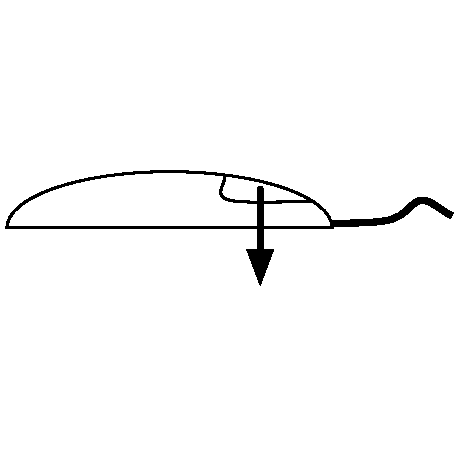
\includegraphics[origin=c, width=5.5cm]{img/button-force-mouse.pdf} 
}
\hspace{1cm} \subfigure[Pressing a stylus button is likely to cause
  accidental pen tip movement.] {
    \label{fig:button-force-pen}
    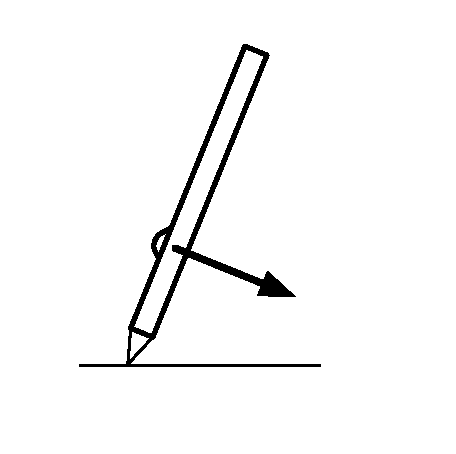
\includegraphics[origin=c, width=5.5cm]{img/button-force-pen.pdf}
}
\caption[Pen vs. Mouse]{The force required to press a mouse button compared with a
  stylus button.}
\label{fig:button-force}
\end{figure}


Some styluses have buttons. While buttons are an indispensable part of
a mouse, they are often difficult to use on the barrel of a
pen~\cite{plimmer-pen-usability}. The force of a \textit{mouse} button
click is orthogonal to the device's plane of use and has negligible
effect on target accuracy. However, pressing buttons on a
\textit{stylus} can move the tip of the pen, making it difficult to
accurately press the button while pointing at particular objects (see
Figure~\ref{fig:button-force}). Further, pressing a button on a
computer stylus usually requires the user to adjust the pen in
hand. This action may be distracting and uncomfortable for long term
use.

\section{Sketching Systems for Fabrication}

\textit{Sketch It, Make It} is a sketch-based tool for rapid
fabrication. This section discusses similar design tools that let
people design objects for physical fabrication. 

Makers of physical things sketch throughout their process. In the
early phases, sketching is used to explore ideas, develop concepts,
and gradually give detail as the final product comes into
focus. Later, people annotate renderings and blueprints with freehand
edits to indicate desired changes. An example of late-phase sketching
is shown in Figure~\ref{fig:late-phase-annotate}. There is a strong
tradition in physical design domains to sketch throughout the
process---from concept generation through fabrication.

\begin{figure}[t]
  \centering
  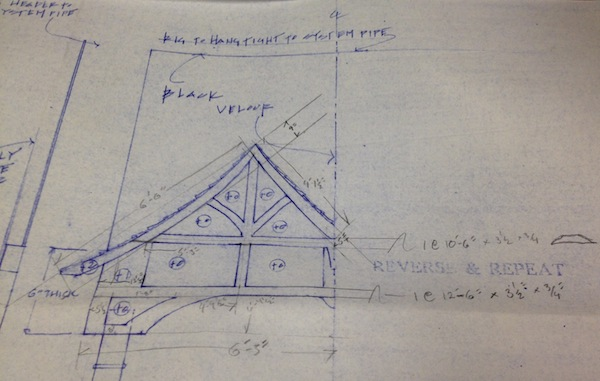
\includegraphics[width=4in]{img/late-phase-hand-annotation.jpg}
  \caption[Annotating a Blueprint]{Designers, builders, and clients
    annotate a formal blueprint with desired changes during the final
    stages of production. The drawing serves as a context for
    stakeholders to communicate with one another, with modifications
    sketches by hand.}
  \label{fig:late-phase-annotate}
\end{figure}


Designers often create perspective drawings of 3D objects. This is a
common activity on paper, so it is an appealing activity to
support. There are two primary approaches to sketching 3D objects:
either draw in perspective, or draw 2D planar diagrams that correspond
to a 3D product. Some researchers combine these approaches.

In the first set (perspective drawing), some systems focus on giving
the designer interaction techniques to form 3D
shapes~\cite{kara-3d-styling,bloomenthal-sketch-n-make}, while others
attempt to infer the 3D shape using statistics and perceptual
rules~\cite{lipson-correlation}. 

The second set (convert 2D drawings to 3D objects) is a natural fit
with domains where the finished product is composed of flat
sheets. Oh's \textit{Furniture Factory}~\cite{oh-fab}, and Saul and
\textit{et. al}'s \textit{SketchChair}~\cite{saul-sketch-chair} tools
let designers draw and fabricate furniture. Sketching is done in a 2D
window, and is mapped to a 3D representation that lets the user see
their composition. In both systems, the system uses domain knowledge
to make the process possible. For example, Furniture Factory will
create appropriate joints where two parts meet. SketchChair does the
same while adding a physics and ergonomic simulation to see if the
chair will fall over and be comfortable to sit in.

A combined approach is demonstrated in
\textit{Plushie}~\cite{mori-plushie}. The user designs plush toys in a
3D environment similar to Teddy~\cite{igarashi-teddy} and applies
textures as desired. The shape will eventually be fabricated from
actual cloth, involving cutting and sewing. Plushie shows the user the
2D cutout patterns associated with the 3D model. These cutouts can't
be edited directly, but it does give a sense of how much work is
involved with physical production.

In contrast with the systems mentioned above, Song's
\textit{ModelCraft}~\cite{song-modelcraft} system lets designers
sketch on physical objects to edit virtual models. The objects are
covered in (or composed of) Anoto paper. This paper has a dot pattern
that is visible to a special pen that identifies where the pen is
drawing. ModelCraft users can annotate or edit virtual objects using
different color ink. 

\section{Sketch Recognition}

Recognition is the centerpiece of many software prototypes that
support sketching. Although the research focus of many systems is not
recognition, such systems use automatic interpretation of sketches to
explore methods to interact with computers and new ways to
design~\cite{gross-boe,grundy-maramasketch,lin-denim}. Such projects
rely on reasonably accurate recognizers. Recognition is therefore a
topic that affects nearly all aspects of research on sketch-based
systems. For this reason, a substantial portion of this document is
devoted to aspects of sketch recognition. This includes timing issues,
determining what to recognize and how those elements can be
recognized, and interaction issues (see Table
\ref{tab:recognition-topics}).

\begin{table}
\begin{tabular}{p{5cm}| p{2cm} | p{8.5cm}}
\textbf{Topic} & \textbf{Section} & \textbf{Remark} \\
\hline \hline
Recognition accuracy &
\ref{sec:recognition-accuracy} & Discusses how to measure recognition 
accuracy, and what acceptable error rates are.
\\ \hline
When to recognize & 
\ref{sec:recognition-when} &
Recognition is powerful but may also distract users from their
task. 
\\ \hline
What to recognize &
\ref{sec:recognition-what} & Sketches may represent objects
(e.g. tables and chairs) and spatial or functional relationships
between those objects (e.g. chairs positioned around table perimeter).
\\ \hline
How to segment &
\ref{sec:recognition-segmentation} &
Sketches contain many different symbols that may overlap. Recognizers
must isolate groups of marks for consideration.
\\ \hline
How to recognize &

\ref{sec:recognition-techniques}, \ref{sec:recognition-hard-coded},
\ref{sec:recognition-library} &

Many recognition techniques exist, and rely on segmentation
methods. \\ \hline

Mediating recognition error &
\ref{sec:recognition-managing-ambiguity} &
Recognition often results in ambiguous results.
\\ \hline

\end{tabular}
\caption[Sketch Recognition Topics]{Topics in sketch recognition}
\label{tab:recognition-topics}
\end{table}


\subsection{Recognition Accuracy}
\label{sec:recognition-accuracy}

Recognition accuracy is typically measured by the deviation between
what the user intended and the machine's interpretation. \textit{Error
  tolerance} refers to the recognition inaccuracy rate a user is
willing to accept. One study using a typewriter modified to make
occasional errors found that typists do not notice a word 0.5\% error
rate, 1\% is manageable, but 2\% is
unacceptable~\cite[p. 79]{cole-survey}. 

It is unclear if there are similar accuracy thresholds for sketching,
though studies have been conducted for related recognition tasks. For
handwriting recognition, adults find 3\% minimally acceptable, with
1\% considered ``very
good''~\cite{lalomia-recognition-accuracy}. Another study examining
user acceptance of hand gesture recognition error rates found users
would tolerate mis-recognition up to 10\% when equivalent keyboard
commands could be employed~\cite{karam-gesture-recognition}.

This is a substantial spread in acceptable error tolerance rates: 1\%
for typewriters, 3\% for handwriting recognition, and 10\% for hand
gestures. One possible explanation is that people have higher
expectations for typewriters (where there is a direct, deterministic
mapping between input and output) compared with recognition based
interaction, because we understand that it is possible the system
might not understand.

\subsection{When to Invoke Recognition}
\label{sec:recognition-when}

It is important that sketching systems \textit{aid} design exploration
and not simply \textit{computerize}
it~\cite{negroponte-soft-arc-mac}. For example, a sketch recognition
system might zealously identify parts of the user's drawing as it is
made, replacing the rough sketch with lines or curves. This removes
the opportunity for reflection and re-interpretation that is so
important to the early phases of
design~\cite{schon-reflective,goldschmidt-dialectics,terry-creative-ui}. Premature
recognition may interrupt the designer's flow of thought and interfere
with the task at hand. Instead we may want the computer to eavesdrop
silently, and provide help only when we need it.

A system can provide the user feedback of sketch recognition on
different occasions: (1)~in mid-stroke, (2)~immediately after the pen
is lifted, (3)~when the system infers that feedback may be
appropriate, (4)~only upon request, or (5)~never. Many interfaces
attempt immediate recognition of gestures for invoking commands, such
as with marking menus~\cite{kurtenbach-marking-menus} or PDA device
character input~\cite{palm}. This is commonly called \textit{eager}
recognition~\cite{blostein-diagrams-review}. Other
systems~\cite{gross-ecn-uist,igarashi-suggestive,alvarado-sketchread-uist}
perform recognition in the background, deferring judgment until
adequate information is available. This is termed \textit{lazy}
recognition. Most modern research prototypes take this approach. Last,
some systems wait until the user explicitly requests
recognition~\cite{landay-silk}, or avoid recognition
entirely~\cite{forbus-nusketch-battlespace}. Combinations of these
approaches are common.

\subsection{What Should be Recognized}
\label{sec:recognition-what}

Different kinds of design drawings (``model ink'') in many domains
might be recognized: artistic sketches, study sketches, drawings,
diagrams, schematics, blueprints, and so on. In addition to model ink
comprising those drawing types, user input may be interpreted as a
command (``command ink''). The particular rules about what should be
recognized depends on the domain (architecture or circuit design),
kind of model (floor plan or timing diagram), and other
application-specific requirements. Sketches often contain hand-written
labels or annotations, which are common targets of pen based
recognition.

% TODO: make the above paragraph SIMI-specific

Diagrams usually have a domain-specific grammar describing how
vocabulary items relate~\cite{lakin-vmacs-89}. For example, boxes may
connect to other boxes via lines, those lines may have arrowheads to
indicate direction. Diagrams are good candidates for recognition
because the various elements and their relations can be described
formally. Table \ref{tab:what} summarizes various recognizable
classes.

\begin{landscape}
\begin{table}
\begin{tabular}{ p{4cm} | p{4.5cm} | p{5.5cm} }
\textbf{``What'' to recognize} & 
\textbf{Examples} & 
\textbf{Remark} \\ 
\hline \hline

Genre &
Mathematical graph, architectural floor plan, web site layout, circuit design &

It may be sufficient to recognize a sketch is of a certain kind
without asking the user. The program could assume the sketch is
in a certain domain.\\ \hline

Characters (writing) & 
Alphanumerics, math symbols & 
Usually with other characters, in words and sentences. \\ \hline

Geometric shapes & 
Dots, lines, rectangles, blobs &
Geometric shapes are often drawn in relation to others. \\ \hline

Spatial features &
A is contained in, is above, is larger than B &
Spatial relations among elements may influence recognition. \\ \hline

Entities &
Domain-specific notation such as diodes, transistors &
Contextual clues can help disambiguate semantics of domain symbols. \\ \hline

Artistic nuance &
Shadows, textures, color &
Ink that modifies an existing element, perhaps suggesting 3D shape. \\ \hline

Commands &
Object selection, delete, copy, move, etc. &
Command ink specifies operations on the drawing. \\ \hline

Intention &
Drawing's function or behavior, e.g. \textit{circuit breaker} & 
Requires detailed domain knowledge and reasoning. \\ \hline

\end{tabular}
\caption[Elements to Recognize]{Kinds of elements to be recognized}
\label{tab:what}
\end{table}
\end{landscape}


% TODO: make the table relevant to SIMI

\subsection{Segmentation and Grouping}
\label{sec:recognition-segmentation}

Segmentation and Grouping are related processes of breaking down user
input and finding related ink. Segmentation involves partitioning
undifferentiated sketch input into parts (analogous to identifying
word boundaries in speech recognition~\cite{cole-survey}). Grouping is
the process of forming logical collections of data (analogous to
determining which spoken words compose a phrase or sentence).

It is sometimes appropriate to break apart continuous pen strokes into
multiple segments, for example in recognizing letter boundaries in
cursive writing, or finding corners in continuous pen
strokes. Alternately, it may be necessary to group related strokes to
recognize compound objects such as a triangle drawn with three
distinct strokes. To further complicate matters, there may be a number
of reasonable ways to segment user input~\cite{mankoff-burlap}, based
on information such as pen speed, stroke order, perceptual qualities,
domain knowledge or curvature~\cite{kim-segmentation}.

The technical challenge is simplified if the system requires users to
complete each symbol before moving on to another, or if each symbol
must be drawn using a conventional stroke order. However, such
requirements work against the goal of supporting unconstrained, fluid
sketching.

A common and effective method for segmenting ink incorporates time
data. Sezgin's approach combines stylus velocity with curvature to
identify locations of interest such as corners, or places where the
drawer may be taking extra care to be precise
~\cite{sezgin-early-processing,davis-siggraph-tutorial}. Wolin's
MergeCF corner finder extends this approach by initially over-fitting
the stroke with corners and iteratively removing them to arrive at a
better fit. SIMI's ink processing algorithm is based on these.

It is often useful to organize drawn input at higher levels before
performing semantic recognition.  Gestalt psychologists offer the
\textit{laws of perceptual organization} to explain how people make
sense of visual scenes. Humans perceive scenes not only using what is
shown but also with ``invisible extensions as genuine parts of the
visible''~\cite{arnheim-visthink}. The rules of perceptual
organization include \textit{proximity}, \textit{similarity},
\textit{closure}, \textit{continuation} and \textit{common
  fate}~\cite{kanizsa-gestalt} (see Figure~\ref{fig:gestalt}). All of
these features are used by SIMI's sketch recognition system.

\begin{figure}
\centering
  \subfigure[] { 
    \label{fig:gestalt-proximity} 
    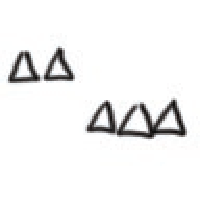
\includegraphics[width=2cm]{img/gestalt-proximity.pdf} 
  }
  \hspace{2mm}
  \subfigure[] { 
    \label{fig:gestalt-similarity} 
    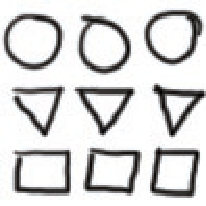
\includegraphics[width=2cm]{img/gestalt-similarity.pdf}
  }
  \hspace{2mm}
  \subfigure[] { 
    \label{fig:gestalt-symmetry} 
    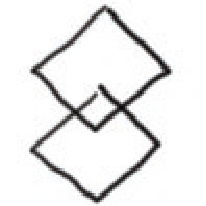
\includegraphics[width=2cm]{img/gestalt-symmetry.pdf}
  }
  \hspace{2mm}
  \subfigure[] { 
    \label{fig:gestalt-continuation} 
    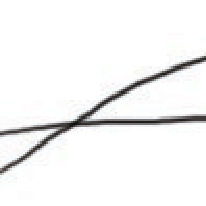
\includegraphics[width=2cm]{img/gestalt-continuation.pdf}
  }
  \hspace{2mm}
  \subfigure[] { 
    \label{fig:gestalt-closure} 
    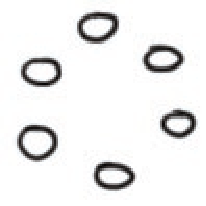
\includegraphics[width=2cm]{img/gestalt-closure.pdf}
  }

\caption[Gestalt perceptual organization]{Some principles of
  perceptual organization~\cite{kanizsa-gestalt}.
  \subref{fig:gestalt-proximity} Proximity: elements near one another
  are seen as belonging to a group. \subref{fig:gestalt-similarity}
  Similarity: objects sharing features such as shape belong in the
  same group. \subref{fig:gestalt-symmetry} Symmetry: two shapes
  symmetric about horizontal and vertical axes, suggesting they belong
  together. \subref{fig:gestalt-continuation} Continuation: the
  simplest explanation is two straight lines, not four lines meeting
  in the middle. \subref{fig:gestalt-closure} Closure: A large circle
  emerges from an arrangement of smaller circles.}
\label{fig:gestalt}
\end{figure}


Perceptual organization supports grouping at many levels. At a
low-level, we can use perceptual rules to analyze the relationship
among individual ink strokes to find plausible groupings for
recognition. PerSketch and ScanScribe explore how perceptual
organization rules can be used at higher
levels~\cite{saund-persketch,saund-perceptual}. 

\subsection{Overview of Recognition Techniques}
\label{sec:recognition-techniques}

Regardless of the input device, we identify two broad categories of
sketch recognition: \textit{on-line} and \textit{off-line}. On-line
recognition knows how fast and in which order marks are made, and is
performed as the drawing is made. Off-line recognition happens after
the drawing is complete, irrespective of the order or speed strokes
were made. SIMI uses on-line recognition.

On-line recognition strategies are further divided in two categories:
single-stroke and multi-stroke recognizers. Single-stroke recognizers
are appropriate for tasks such as interpreting freehand
gestures. Single-stroke approaches are simpler to implement than
multi-stroke strategies because user input is clearly divided into
pieces. This process could be relatively simple: a multi-stroke
recognizer might simply expect multi-stroke objects to be drawn in a
prescribed fashion. Or, multi-stroke recognizers might be more
complex, for example calculating the likelihood that distinct strokes
(or segments) belong together. SIMI uses both single- and multi-stroke
recognizers.

\subsection{Hard-coded Recognizers}
\label{sec:recognition-hard-coded}

One common approach is to hard-code recognition routines directly. For
simple or limited graphical vocabularies this may be appropriate. A
circle (or a zero, or the letter 'O', or the sun, etc.)  can be
recognized with a short program looking for input points that are
roughly equidistant from the stroke's centroid. However, ad-hoc,
hard-coded recognizers are difficult to maintain and extend. For
example, if we wished to extend our circle recognizer to interpret a
sun with rays of light coming out of it, we would have to also
recognize lines, then coordinate the recognizer to consider those
particular lines together with the circle, and ensure that the lines
are positioned and angled correctly. Further, sketch recognition
applications must be able to discern different kinds of
elements. Recognizers for these elements may conflict. A new
recognizer may cause an existing recognizer to stop working correctly,
leading to maintenance, debugging, and testing problems.

SIMI uses hard-coded recognizers in situations when performance is
critical (e.g. erasing and undo/redo).

\subsection{Pattern Matching}
\label{sec:recognition-library}

Another strategy for representing classes is to create a library of
pattern templates. These approaches can be separated into two groups:
those that use \textit{visual} templates, and those that use
\textit{textual} templates.

Template matching strategies are often
\textit{feature-based}. Features include properties such as stroke
length, stroke path, minimum or maximum angle, or aspect ratio. The
system holds a library of templates, each of which has feature
values. The system computes feature values for user input, and
compares those values with those contained in the library. SIMI uses
textual templates, but not the visual kind.

Examples of the visual template method include the Ledeen
recognizer~\cite{newman-sproull-graphics-2}, the Rubine
recognizer~\cite{rubine-recognizer}, Kara's
recognizer~\cite{kara-recognizer-cg}, and the \$1
Recognizer~\cite{wobbrock-dollar}.

Textual templates may be described using a programming
language~\cite{pasternak-adik,bimber-sketch-bnf,costagliola-xpg,hammond-ladder}. These
notations have two primary strengths. First, humans can read (and
edit) them. For example, a television symbol may be described with
natural language as ``a square with a slightly smaller circle
positioned at its center.'' A formal symbolic language for that
statement is still quite legible (assuming one understands the
function semantics):

\begin{verbatim}
      (define television 
              (and (centered square circle)
                   (slightly-smaller circle square)))
\end{verbatim}

Another strength of this kind of notation is that it allows the
developer to describe entities at a level of abstraction that
accommodates variability between entity
instances. An \textit{abstract} triangle is a three-sided,
two-dimensional shape whose internal angles add up to
180$^\circ$. A \textit{particular} triangle may have side lengths of 3,
4, and 5, and be oriented so that its long edge is horizontal. We may
define triangles and other entities as abstractly or concretely as the
language allows.

Many of the recognizers in SIMI use textual templates roughly based on
the approaches described by Hammond~\cite{hammond-ladder} and
Alvarado~\cite[Chapter 4]{alvarado-phd-thesis}.

\subsection{Managing Ambiguity}
\label{sec:recognition-managing-ambiguity}

Futrelle's classification scheme of types of ambiguity in diagrams
includes two high-level categories: lexical and structural
ambiguity~\cite{futrelle-ambigutiy}. Lexical ambiguity refers to the
``word'' level, when the meaning of a particular symbol is in
question. Structural ambiguity refers to confusion arising from the
composition of symbols.

Shilman augments this scheme with two additional types of ambiguity
that arise in sketch recognition: label and attribute
ambiguity~\cite{shilman-parsing}. Label ambiguity is present when the
symbol's identity is unclear. For example, a quickly drawn rectangle
might be interpreted as a circle. Attribute ambiguity refers to the
features of a sketched element: the exact location of a quickly drawn
rectangle's corner may be unclear.

BURLAP~\cite{mankoff-burlap} is a calligraphic application based on
SILK~\cite{landay-silk} that enables people to draw user
interfaces. As the user draws, BURLAP forms a list of plausible
interpretations. At some point the system may need to pick one
interpretation. Mankoff \textit{et. al} call this process
\textit{mediation}, performed by agents called
\textit{mediators}. Some mediators may engage the user by displaying a
pick-list of choices or visually indicating the ambiguity. Other
mediators automatically execute and do not involve the user. SIMI
uses this automatic way to disambiguate contending interpretations.

Another way to manage ambiguity is to prevent it from arising in the
first place. Some sketching systems let designers model 3D
objects. Recognizing 3D topology from a 2D sketch is difficult because
of \textit{Z ambiguity}: for any point on the $(x, y)$ plane, there is
an infinite number of possible $z$ values. In Kara's automotive
styling system~\cite{kara-3d-styling}, designers use specific
sketch-based interaction techniques to achieve unambiguous $z$
values. By contrast, Lipson's 3D modeling sketching
tool~\cite{lipson-correlation} does not impose special techniques on
the user, and instead attempts to derive $z$ values by searching a
space of possible interpretations weighted by past observations of
3D-to-2D reverse projections.

The two 3D modeling systems described in the preceding paragraph use
different approaches to manage ambiguity: In Kara's system, the
approach is interaction design; in Lipson's, it is based on perception
and statistics. Researchers have found success with both
approaches. SIMI is entirely based on interaction design.

